\documentclass[12pt, cjk, dvipdfmx]{beamer}
% 縦向き : orientation=portrait, 横向き : orientation=landscape
\usepackage[orientation=portrait,size=a1,scale=1.9]{beamerposter}
% パッケージ
\usepackage{here, amsmath, latexsym, amssymb, bm, ascmac, mathtools, multicol, tcolorbox, enumerate}
\usepackage{graphicx} % 図を表示するためのパッケージの追加                                           
\usepackage{bm} % 太字イタリックを使えるようにする
\usepackage{caption}


% beamer に関する設定                                                                                
% Adobe Reader の文字化けを防ぐおまじない                                                            
\AtBeginDvi{\special{pdf:tounicode EUC-UCS2}}

\usecolortheme{orchid}           %カラーテーマの選択(省略可)
\usefonttheme{professionalfonts} %フォントテーマの選択(省略可)
\useinnertheme{circles}          %フレーム内のテーマの選択(省略可) 
\setbeamertemplate{navigation symbols}{} %ナビゲーションバー非表示
\renewcommand{\kanjifamilydefault}{\gtdefault} %既定をゴシック体に


%itemizeの設定
%\setbeamertemplate{itemize item}{\normalsize\raise1.0pt\hbox{$\bullet$}}
%\setbeamertemplate{itemize subitem}{\normalsize\raise1.0pt\hbox{$\blacktriangleright$}}
%\setbeamertemplate{itemize subsubitem}{\normalsize\raise1.0pt\hbox{$\bigstar$}}
\setbeamertemplate{itemize item}{\normalsize\raise0.5pt\hbox{$\bullet$}}
\setbeamertemplate{itemize subitem}{\normalsize\raise1.0pt\hbox{$\blacktriangleright$}}
\setbeamertemplate{itemize subsubitem}{\normalsize\raise1.5pt\hbox{$\bigstar$}}
\renewcommand{\baselinestretch}{1.2}  % 行間設定


% colorの設定
\newcommand{\red}[1]{\textcolor{red}{#1}}
\newcommand{\green}[1]{\textcolor{green!40!black}{#1}}
%\newcommand{\blue}[1]{\textcolor{blue!60!white}{#1}}
\newcommand{\blue}[1]{\textcolor{blue!80!black}{#1}}


%headlineの背景色を変更 fg:多分フォントの色, bg:多分背景の色
\setbeamercolor{headcolor}{fg=white,bg=blue!80!black}

% ヘッダーの設定
% (背景色 白, 文字色 青)
% \setbeamertemplate{headline}{
%     \begin{center}
%         \structure{
%             \vskip2ex
%             \rule{1.0\linewidth}{3mm}
%             \vskip2ex
%             \usebeamercolor{title in headline}{\textbf{\LARGE{\inserttitle}}\\[2.5ex]}
%             \usebeamercolor{author in headline}{\normalsize{\insertauthor}\\[1.2ex]}
%             \usebeamercolor{institute in headline}{\normalsize{\insertinstitute}\\[1.2ex]}
%             \usebeamercolor{date in headline}{\normalsize{\insertdate}}
%             \vskip2ex
%             \rule{1.0\linewidth}{3mm}
%         }
%     \end{center}
% }

% (背景色 青, 文字色 白)
\setbeamertemplate{headline}{
        \begin{beamercolorbox}{headcolor}
          \begin{center}
            \vskip3ex
            \usebeamercolor{title in headline}{\textbf{\LARGE{\inserttitle}}\\[2.5ex]}
            \usebeamercolor{author in headline}{\normalsize{\insertauthor}\\[1.2ex]}
            \usebeamercolor{institute in headline}{\normalsize{\insertinstitute}\\[1.2ex]}
            \usebeamercolor{date in headline}{\normalsize{\insertdate}}
            \vskip3ex
          \end{center}
        \end{beamercolorbox}
}


% フッターの設定
\setbeamertemplate{footline}{
    \begin{center}
      \structure{
          \rule{1.0\linewidth}{2mm}
          \vskip2.5ex
          \begin{columns}[T]
              \begin{column}{0.65\paperwidth}
              \end{column}
              \begin{column}{0.35\paperwidth}
                  \usebeamercolor{conference in headline}{\normalsize{\foot}}
              \end{column}
          \end{columns}
          \vskip2.5ex
      }
  \end{center}
}


% ブロック(ボックス)の設定 (tcolorboxで検索かければ色々出てくる)
\newtcolorbox{mybox}[1]
{
    title=#1, 
    toptitle=2mm, bottomtitle=2mm, 
    colframe=structure,boxrule=3pt,
    coltitle=white, colbacktitle=structure,
    colbacktitle=blue!80!black, sharp corners,
    colback=blue!10!white, fonttitle=\bfseries\large, % fonttitle:タイトルのフォントの設定
    top=4mm, bottom=5mm, left=1.0mm, right=1.0mm, %内部余白調整
    enlarge top by=0.8mm, enlarge bottom by=0.8mm,
    enlarge right by=0.5mm, enlarge left by=0.5mm %外部余白調整
}


% タイトル部分の設定 {}の中を自分用に書き換えるだけでおk
\title{Artificial Bee Colonyアルゴリズムによるサポートベクトルマシンのハイパーパラメータ最適化}
\author{2131007 安達拓真}
\institute{千葉工業大学 情報科学部 情報工学科 4年}
\date{2024年9月3日}
% フッターに表示される内容
\newcommand{\foot}{千葉工業大学 情報工学科 山口研究室} 


% 文書本文
\begin{document}
  \begin{frame}
  % 表示領域の調整
  \vspace{-1.4cm}
  % 二つのコラム(左と右)でポスターを構成
    \begin{columns}[t]
        % 左側のコラム
        \begin{column}{0.490\linewidth}
            % \begin{mybox}{タイトル名} 内容 \end{mybox}
            \begin{mybox}{はじめに}
                % 箇条書き
                \begin{itemize}
                  \item 機械学習にはハイパーパラメータがある
                  \begin{itemize}
                    \item 手動での調節は時間を要する
                    \item 自動調節のための手法が提案されている
                  \end{itemize}
                  % \item サポートベクトルマシン(SVM)の\\ハイパーパラメータ最適化
                  \item サポートベクトルマシン(SVM)における自動調節
                  \begin{itemize}
                    \item Artificial Bee Colony(ABC)アルゴリズムを適用した研究
                  \end{itemize}
                  \item 本研究ではカーネル関数も最適化対象とする
                  \begin{itemize}
                    \item SVMの分類精度向上を図る
                  \end{itemize}
                \end{itemize}
            \end{mybox}
            \begin{mybox}{サポートベクトルマシン(SVM)}
                \begin{itemize}
                  \item 機械学習アルゴリズムの一つ[1]
                  \begin{itemize}
                    \item 主に分類問題に使用される
                  \end{itemize}
                  
                   %  ここも図がほしいです
        
                  \item カーネルトリックを使用して、非線形データを高次元空間に写像し、線形分離可能にする 
                  \item データを分類する最適な境界線(超平面)を探す                
                \end{itemize}
                \begin{figure}
                  \centering
                  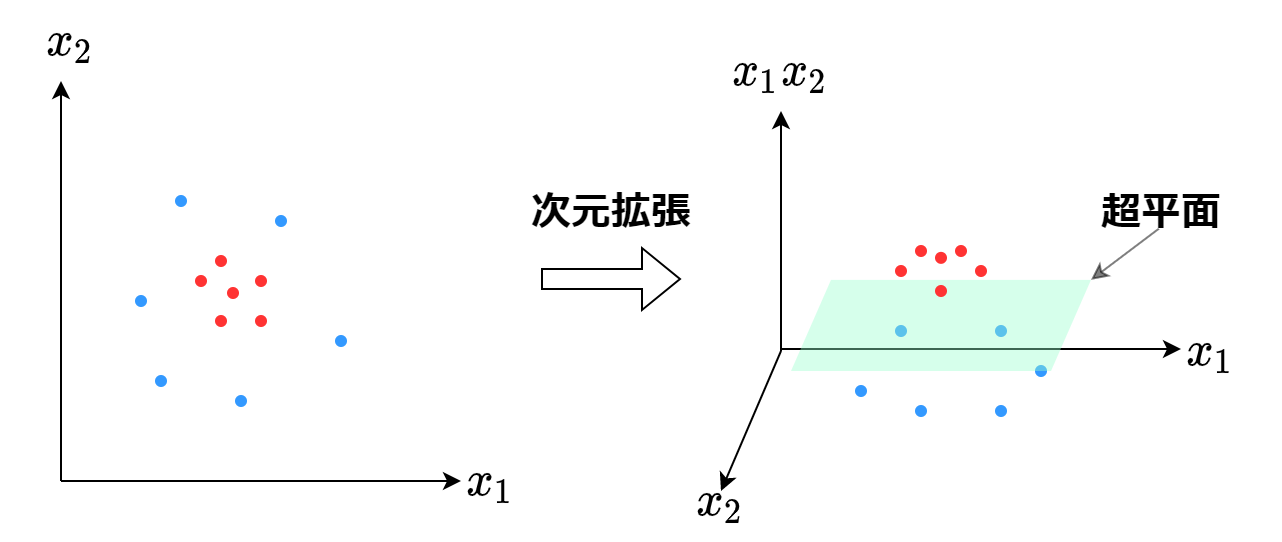
\includegraphics[width=0.9\linewidth]{syazou.png}
                  \caption{高次元空間への写像の例}
                 \end{figure}
            \end{mybox}
            \begin{mybox}{ハイパーパラメータ最適化(HPO)}
              \begin{itemize}
                %いらないかも
                \item 機械学習の性能を最大限に発揮するには適切な\\ハイパーパラメータの選択が必要不可欠
                \item 手動で経験的に決めることが多い
                \item HPOは一般的に計算量が大きい
                \begin{itemize}
                  \item 効率的なパラメータ空間の探索が必要
                \end{itemize}
                \item ハイパーパラメータの性質は様々
                \begin{itemize}
                  \item 離散値
                  \item 連続値
                  \item カテゴリ変数
                \end{itemize}
              \end{itemize}
            \end{mybox}
            \begin{mybox}{Artificial Bee Colony(ABC)アルゴリズム}
              \begin{itemize}
                \item 蜂の採餌行動に着目した最適化アルゴリズム[2]
                \item 働き蜂、追従蜂、偵察蜂の三種類の蜂によって各個体(食物源)の探索を行い、最適解を求める
                %\item 連続値の最適化を前提としている
                \item ABC自体の設定パラメータは少ない
              \end{itemize}
          \end{mybox}
        \end{column}
        % 右側のコラム 
        \begin{column}{0.490\linewidth}
          
          \begin{mybox}{先行研究}
            \begin{itemize}
            % \item SVMのカーネル関数をRBFに固定した上で、ABCアルゴリズムを用いてSVMのハイパーパラメータの最適化とデータセットの特徴選択を行った[3]
            \item SVMのハイパーパラメータの最適化とデータセットの特徴選択にABCを適用[3]
            \begin{itemize}
              \item カーネル関数はガウスカーネルに固定
            \end{itemize}
            \end{itemize}
          \end{mybox}
          \begin{mybox}{問題点}
            \begin{itemize}
            \item カーネル関数を1つに固定している
             \begin{itemize}
            \item  カーネル関数には様々な種類がある
             \end{itemize}
            \item カーネル関数によってハイパーパラメータは異なる
               \begin{itemize}
                  \item ハイパーパラメータ空間の探索範囲が限定的
               \end{itemize}
            \end{itemize}
          \end{mybox}
           
            \begin{mybox}{提案手法}
              \begin{itemize}
                \item 4つのカーネル関数とそのハイパーパラメータも最適化対象とする
                \item 最適化アルゴリズムはABCアルゴリズムを利用
                \item 解は5次元のハイパーパラメータの組で表す
                  \begin{itemize}
                    \item (カーネル関数, C, gamma, coef0, degree)                   
                  \end{itemize}
                \item ハイパーパラメータの扱い
                  \begin{itemize} 
                  \item gamma, coef0, degreeの3つはカーネル関数によって異なる
                  \begin{itemize}  
                    \item 選択されたパラメータのみを更新の対象にする
                  \end{itemize}    
                  \item カーネル関数は4種類の値をとるカテゴリ変数
                  \begin{itemize}
                    \item 整数にエンコード
                    \item 更新はランダムに選ばれた個体とのルーレット選択
                  \end{itemize}
                \end{itemize}
              \end{itemize}
              \begin{align*}
                P = \frac{f(x_j)}{f(x_i)+f(x_j)}
               \end{align*}
               \begin{itemize}
                \item 探索範囲を広くし、より最適なSVMモデルの探索を可能にする
              \end{itemize} 
              \begin{align*}
             \text{線形カーネル: }  K(x, x') &= x \cdot x'\\
             \text{多項式カーネル: }   K(x, x') &= (\gamma \, x \cdot x' + \text{coef0})^d\\
             \text{ガウスカーネル: }   K(x, x') &= \exp(-\gamma \, \|x - x'\|^2)\\
             \text{シグモイドカーネル: }  K(x, x') &= \tanh(\gamma \, x \cdot x' + \text{coef0})
               \end{align*}
            \end{mybox}
            
           %  \begin{mybox}{今後の予定}
            %   \begin{itemize} 
            %     \item プログラムの実装
            %     \item ライブラリデフォルトのパラメータと提案手法で最適化したパラメータの比較
             %    \item 既存研究との比較
             % \end{itemize}
           %  \end{mybox}
            \begin{mybox}{参考文献}
              %\footnotesize
              \scriptsize
              \begin{description}
                \item[{[1]}] Cortes, C. and Vapnik, V. Support-vector networks, Ma-chine Learning, Vol.20, No.3, pp.273-297, 1995.
                \item[{[2]}] Karaboga, Dervis. An idea based on honey bee swarm for numerical optimization. Vol. 200. Technical report-tr06, Erciyes university, engineering faculty, computer engineering department, 2005.
                \item[{[3]}] 近藤 久,浅沼 由馬“人工蜂コロニーアルゴリズムによるランダムフォレストとサポートベクトルマシンのハイパーパラメータ最適化と特徴選択”,人工知能学会論文誌, vol34-2, pp.1-11, 2019.
              \end{description}
            \end{mybox}
        \end{column}
      \end{columns}
  \end{frame}
\end{document}